\documentclass[english]{article}
\usepackage[T1]{fontenc}
\usepackage[latin9]{inputenc}
\usepackage{color}
\usepackage{amsmath}
\usepackage{amssymb}
\usepackage{esint}
\usepackage{babel}
\usepackage{graphicx}

\begin{document}
\title{\vspace{-4.5ex} \large{\textbf{\MakeUppercase{Finite Differences Schemes for PDE}}}\vspace{1ex}}
\author{\large{\textsc{Matthieu Gomez}}}
\date{\today}
\maketitle
\tableofcontents
\newpage

\section{Write Monotonous Scheme}
\begin{itemize}
	\item 	Barles Souganadis theorem
	Take the following PDE
	$$0 = u_t + F(t, x, v, \partial v, \partial^2 v)$$
	with F elliptic, i.e.if $X - Y$ positive semi definite
	$S(x, v, \partial v, X) \geq S(x, v, \partial v, Y)$
	Denote a scheme a function 
	$$0 = S(\Delta a, v_j^{n+1} ; ...)$$
	A scheme is convergent if it is decreasing in all variables in ..., i.e.  typically $v_{i+1}^{n+1}, v_{i-1}^{n+1}, v_{i+1}^{n}, v_{i}^{n}, v_{i+1}^{n}$  (i.e. all values except potentially $v_j^{n+1}$)
	\item Interpretation in term of  monte carlo chain
	For The PDE
	$$\rho V = f(x, u) + \alpha(x, u) DV(x) + \sigma^2(x, u) D^2 V(x)$$
	A fully explicit finite difference schemes can be rewritten
	$$V =  V + \Delta f(x, u) + \sum p(x_k, y|u)V^h(y) $$
	where $p(X_k, y|u) \geq 0$.  An explicit monotonous scheme can be interpreted in term of a monte carlo chain.
	A monte carlo chain approximates the solution if it is consistent (denonting markov chain $\xi^h_n$)
	$$E\Delta \xi = b(x) \Delta T$$
	$$Var\Delta \xi = \sigma^2 (x) \Delta T$$
\end{itemize}

\subsection{Monotonous Scheme for first derivative}
$$\rho V = f(V, x) + m(x) \partial V + a(x) \partial^2V$$ 
How to satisfy monotonicity ?
\begin{itemize}
	\item Monotinicity in $v_{j+1}$ and $v_{j-1}$ by upwinding
	$$S =-\rho v_{n+1, j} + f(x_j) + \frac{v_{j+1}-v_{j}}{\Delta a} m(x)^+ - \frac{v_j-v_{j-1}}{\Delta a} m(x)^-$$
	$$S =-\rho v_{n+1, j} + f(x_j) + \frac{v_j-v_{j-1}}{\Delta a} c_{j, B} - \frac{v_{j+1}-v_j}{\Delta a} (w + ra_j)$$
	Economic interpretation:  savings are positive, what matters is how the value function changes when wealth increases by a small amount; and vice versa when savings are negative. The right thing to do is therefore to approximate the derivative in the direction of the movement of the state.
	\item Monotinicity in $v_{j}$. $v_j$ appears negatively in first and second derivative term. Thus does not satisfy Barles Souganadis theorem.
	\begin{itemize}
		\item One solution consists in adding a time derivative at the LHS. Then this counterbalances the negative term by a $\frac{1}{\Delta t}$. 
		The issue is that, so that scheme is monotonous wrt $v^n_t$, one needs to bpick $\Delta t$ low enough. This forces the time step to be so small	that the rounding error dominates the total computational error
		\item Another solution consists in replacing everything by $n+t$ (explicit scheme)
		\begin{itemize}
			\item If $f$ is linear in $v$ then replace by $v^{n+1}$ here too
			\item If $f$ is monotone in $v$, then use $v^n$ there. This includes case of optimal policy in $v$ by envelop theorem.
			\item The resulting scheme is monotonous Why? envelop theorem.
			\item     One caveat: you have to make sure you're using the same derivatives to compute the control and in the rest of the PDE so that envelop theorem applies.
			Since $v$ is generally concave in $a$, $s_F \leq s_B$, where $s_F$ is the drift computed using forward difference for consumption and $s_B$ the backward. Therefore the following situation happens: positive difference for $\partial V$ when computing $c$ gives negative drift, while positive difference gives positive drift). For these grid points, set the derivative of the value function equal to the case where drift is zero (i.e stationary value)
			\item This circularity becomes too complicated with multiple controls . In this case, split the drift in two
			$$S = \rho v_j - u(c_j) + \frac{v_j-v_{j-1}}{\Delta a} c_{j, B} - \frac{v_{j+1}-v_j}{\Delta a} (w + ra_j)$$
			It is done in the Moll notes with fixed cost
			\begin{align*}
				\rho V =\max_c u(c) + V_b(r^b-\chi(d, a) - c) + V_a(r^a a + d)
				V_b \chi_d(d, a) = V_a
			\end{align*}
		\end{itemize}
		\item If $f$ is non linear in $v$ and non monotonous, this requires to use a non linear algorithm
	\end{itemize}
	\item Second derivative
	\begin{itemize}
		\item Naive approximation is
		\begin{align*}
			\partial_{ij}v&=\frac{v_{i+1, j+1} + v_{i-1, j-1} - v_{i+1, j-1} - v_{i-1, j+1}}{4\Delta x^2}
		\end{align*}
		This is never monotonous because the term $v_{i+1, j-1}$ enters negatively and does not appear anywhere else
		\item Better scheme
		\begin{itemize}
			\item If $a_{ij}(x) \geq 0$
			\begin{align*}
				\partial_{ij}v&= \frac{1}{2}(\frac{v_{i+1, j+1} + v_{i-1, j-1}- 2v_{i,j}}{\Delta x_i \Delta x_j} \\
				&-  \frac{v_{i+1, j} + v_{i-1, j}- 2v_{i,j}}{(\Delta x_i)^2}\\
				&-  \frac{v_{i, j+1} + v_{i, j-1}- 2v_{i,j}}{(\Delta x_j)^2})
			\end{align*}
			\item if negative, a classical scheme is
			\begin{align*}
				\partial_{ij}v&= \frac{1}{2}(-\frac{v_{i+1, j-1} + v_{i-1, j+1}- 2v_{i,j}}{\Delta x_i \Delta x_j} \\
				&+  \frac{v_{i+1, j} + v_{i-1, j}- 2v_{i,j}}{(\Delta x_i)^2}\\
				&+  \frac{v_{i, j+1} + v_{i, j-1}- 2v_{i,j}}{(\Delta x_j)^2})
			\end{align*}
			\item This scheme is monotonous when the negative terms in $v_{i+1, j}$ and $v_{i, j+1}$ are compensated by the diagonal terms of the Hessian. More precisely, the scheme is monotonous iff 		$$a_{ii}(x) \geq \sum |a_{ij}(x)|$$
		\end{itemize}
		\item Rewrite in term of directional derivatives. Denote $a(x)$ such that the second order term is $\sum a_{i, j}(x) \delta_{ij} v$.
		\begin{itemize}
			\item If  $a = \sum \lambda_i \xi_i \xi_i$, the second order term can be rewritten only in term of directional derivatives:
			\begin{align*}
				\sum \lambda_i D_\xi^2v
			\end{align*}
			$D_\xi v$ is the directional derivative along the direction $\xi$
			$$D^2_\xi v \approx \frac{v(t, x+\xi \Delta x) + v(t, x-\xi \Delta x) - 2 v(x)}{|\xi|^2 \Delta x^2}$$
			The corresponding scheme is monotonous, similarly to the case with diagonal Hessian. 
			How to find this decomposition?
			\item 
			Bonnans. Choose an order $p$ and solve the problem 
			\begin{align*}
				\min_{\lambda_i}&||a - \sum_{\xi \in \Xi_p} \lambda_i \xi_i \xi'_i||^2\\
				\Xi_p &= \{\xi \in Z^d \text{ s.t. }  \max_i|\xi_i^d| \leq p \}\\
				\lambda_i &\geq 0
			\end{align*}
			$p$ needs to be equal to 5 so that mistake is not too large.
			\item Me. For PDE obtained by HJB only. Denote $\sigma(s_t)$ the matrix such that $ds_t = \mu dt + \sigma dW_t$, the second order term has the form 
			\begin{align*}
				Tr(\sigma\sigma^TD^2V)
			\end{align*}
			The matrix $\sigma\sigma^T$ is symetric therefore diagonalizable. There exists positive $\lambda_i$ and directions $\xi_i$ such that
			$$\sigma\sigma^T = \sum \lambda_i \xi_i \xi_i^T$$ 
			The issue is that $\xi \notin Z^d$. One can rewrite this as a scheme on the grid by using use a linear interpolation to approximate $v(t, x+\beta \Delta x) $ as a weighted average of points of the grid (with positive weights). 
			One can always normalize $v$ so that $v_1 = 1$. In particular, in two dimensions, one only needs to interpolate linearly along the second dimension, which simplifies the code (see \autoref{image2015831195641.png})
			\begin{figure}[htp]
				\centering
				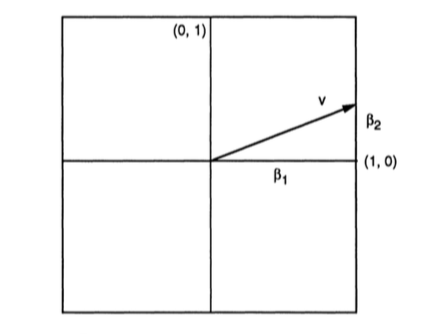
\includegraphics[width=4in]{image2015831195641.png}
				\caption{\label{image2015831195641.png}caption}
			\end{figure}
		\end{itemize}
	\end{itemize}
\end{itemize}

\subsection{Others}

\subsubsection{Discrete maximization}

\begin{itemize}
	\item  Discrete maximiation is handled through splitting method (optimial time / fixed cost).	Suppose there is fixed cost to convert illiquid asset $a$ into liguid asset.	Denote $v^*(w)$ the value function conditionally to paying the fixed cost. It is only a function of wealth.
	\begin{align*}
		v^*(a+b) \equiv \max_{a', b'} v(a', b') \\
		a' + b' * = a + b - \kappa
	\end{align*}
	Then the HJB equation is the same, for $v$ but we have new constraint
	\begin{align*}
		\forall a, b	v(a, b) \geq v^*(a + b)
	\end{align*}
	THis problem is solved in two step
	\begin{align*}
		v^{n+1/2} &\dots \text{(usual HJB)}\\
		v^{n+1}(a', b') &= \max(\max_{a' + b' = a + b - \kappa} v^{n+1/2} (a', b'), v^{n+1/2}(a', b'))
	\end{align*}
\end{itemize}

\subsubsection{Non linear PDE}
$$\rho V = f(x, V) + m(x, \partial V(x)) \partial V(x)+ a(x, \partial V(x)) \partial^2 V(x)$$

\begin{itemize}
	\item Case of ditella $\mu_x$ depends on derivative $\xi_\nu$ etc. The same situation appears when substituting out optimal control by derivative, but in this case the envelop theorem does not apply
	\item Choose different direction in $\partial V(x)$ (even within a grid) for different terms, so that we make sure everything works
\end{itemize}
Is there existence theorem for the scheme?

\subsubsection{Borders}
\begin{itemize}
	\item Upwind scheme has an adantage when using boundary conditions
	\begin{itemize}
		\item saving is negative at the top of state space therefore forward difference is not used and no boundary condition needs to be imposed
		\item since upwind scheme selects a particular derivative when saving (ie drift) is negative, and since condition is about the drift, then we just replace the backward difference derivative by $u'(z+ra_1)$.
	\end{itemize}
	\item First derivative $v_{I+1}-v_{I}$ is handled through upwiding
	\begin{itemize}
		\item Exogeneous state constraint typically does not appear thanks to upwinding (i.e. when we're at the border of state, the drift is mean reverting)
		\item True endogeneous state constraint (like $a \geq 0$) or artificial endogeneous state constraint (like $a \leq a_max$ - not really necessary but "sometimes helps numerical stability") 
		Since FOC holds even at the constraint,  a constraint of $c$ is just a constraint on $v'$.
		$$v'(\underline{a}) \geq u'(z+ r\underline{a})$$
		Note that this constraint binds iff the saving is negative. Thanks to upwind scheme, the boundary condition is therefore
		\begin{align*}
			\partial v^b_1&= u'(z+ r\underline{a})
		\end{align*}
	\end{itemize}
	\item Second derivative  $v_{I+1}+v_{I-1}-2v_{I}$
	\begin{itemize}
		\item if exogeneous mean reverting state variable (like $\mu$), use reflecting barrier $v'(x) = 0$ and therefore  $v_{I+1}=v_I$.
		\item if endogeneous state variable 
		\begin{itemize}
			\item policy funciton $c(a_{max})$ is approximately linear, and so from FOC this allows to express second derivative in term of first derivative 
			$$v''(a_{max}) = -\gamma v'(a_{max})^{1+1/\gamma} \overline{c}$$
		\end{itemize}
	\end{itemize}
\end{itemize}

\section{Method of line}
The idea is to write the explicit system with $t$ non discretized. So instead of writing
$$\frac{v^{n+1}_i -v^{n}_i}{\Delta t} = S(v^{n_i},v^{n_{i-1}},v^{n_{i+1}})$$
you solve the system of $N$ first order ODE
$$\dot{v_i^n} =  S(v^{n_i},v^{n_{i-1}},v^{n_{i+1}})$$
\end{document}